\documentclass[]{auvsi_doc}
\setkeys{auvsi_doc.cls}{
	AUVSITitle={Tail Wedge Design, Construction, and Validation},
	AUVSIRevision=0.0,
	AUVSIDescription={Created},
	AUVSIAuthor={Kameron Eves},
	AUVSIChecker={[Checker]},
	AUVSILogoPath={./figs/logo.pdf},
	AUVSIDocID={AF-004}
}

% include extra packages, if needed
\usepackage{makecell}
\usepackage{longtable}
\usepackage{pdfpages} 

% Remove Heading Numbers
\setcounter{secnumdepth}{0}

\begin{document}
\begin{AUVSITitlePage}
\begin{artifacttable} 
	\entry{AF-009, 0.1, 2-20-2019, Created, Kameron Eves, Tyler Critchfield}
	\entry{AF-009, 0.2, 4-05-2019, System Refinement edits, Tyler Critchfield, Kameron Eves}
\end{artifacttable}

\end{AUVSITitlePage}
\section{Introduction}

During our XFLR analysis detailed in AF-011 we determined that the aircraft would need a significant (-7.5°) horizontal stabilizer incidence angle. The negative incidence angle is very normal in aircraft design and is designed to provided negative lift to push the tail down until the aircraft reaches a trimmed state (i.e. the pitching moment induced by the wings is equal and opposite to the moment induced by the negative lift from the tail). However, the aircraft, as built by the company we purchased it from, has a 0° incidence angle. 

The aircraft can still fly in this configuration; the necessary negative lift is caused by deflecting the elevator up (conventionally negative deflection). This effectively causes the horizontal stabilizer to have decreased (moves from 0 towards negative infinity) camber and angle of attack. This induces a negative lift that trims the aircraft.  However, this is not an ideal configuration as it necessitates flying with constant deflection on the elevator. Because the equilibrium point for the elevator is not at zero, the throw of the elevator is decreased. In other words, the elevator's saturation point is too close to the equilibrium point and we have decreased control authority. Our first couple flight tests validated this analysis as significant negative elevator deflection was necessary to trim the aircraft. Thus we sought another way to induce this negative lift. 

\section{Design}

It was determined that the most effective way to induce this negative lift was to create a wedge that would be mounted between the empennage and the tail of the aircraft. This would give us the required negative incidence angle, but would also decrease the sweep on the vertical stabilizer and adjust the rudder so that it is not exactly orthogonal to the aircraft body. We decided, however, that these were acceptable trade-offs as leading edge sweep only has a positive effect on the aerodynamics (decreasing the drag) if the airspeed of the aircraft is near the speed of sound. Because our design flight speed is significantly below the speed of sound (15 m/s), we decided that decreasing the leading edge sweep of the vertical stabilizer is acceptable.
 
Angling the rudder would have adverse consequences on its effectiveness and cause coupling between the rudder and the pitching moments. However, the developers of the autopilot we are using have found that the rudder provides very little benefit to the aircrafts over all control schemes. The rudder is usually used to mitigate sideslip and allow for coordinated turns, but the the sideslip is usually mitigated sufficiently by having a large horizontal stabilizer (which we do) and coordinated turns are only really beneficial to passenger comfort (something we don't care about as this aircraft will not be carrying passengers). Thus the autopilot we use commands the rudder to be constant at it's trim value (zero or very close to zero) and adjustments to the rudder mounting orientation should have little to no effect on our overall flight characteristics.
 
From the above analysis we decided that a wedge would be mounted between the tail and the empennage. This wedge needed to have a flat bottom to allow it to be glued to the applicable section of the tail and another flat surface 7.5° from the bottom for the tail assembly to be attached to it. Finally, the outer profile of the wedge only needed to match the outer profile of the tail to reduce drag. Artifact AF-010 is a dimensioned CAD drawing showing the wedge shape. Important to note is that the outer profile of the wedge is not dimensioned. The outer shape of the wedge follows the complex profile of the aircraft's tail. For more exact specification, contact the manufacture of the Nimbus Pro aircraft. See the construction shape below for a description of how we manufactured this shape. 
 
Pink insulation foam that can be purchased at any hardware store was chosen as the material for the wedge because it was readily available, cheap, light-weight, and would not have to bare significant forces (the large moment arm of the tail means that the forces necessary to trim the aircraft are small and the wide base of the wedge means that the stresses induced by those forces are even smaller). 

\section{Construction}

The wedge's outer profile was cut to the desired angle by a foam cutter. The raw material was placed in the foam cutter and the custom shape was loaded into the cutting software. The profile cut by the foam cutter only gave the desired angle for the wedge. The outer profile of the wedge was cut by holding the wedge in the position it was to be installed in and tracing the geometry of the tail assembly directly on to the cut wedge. This was then cut again using the foam cutter's heated wire, but this time we manually manipulated the foam to produce the required shape. Light-weight RC aircraft grade glue was used to bind the wedge to the tail and empennage. Figure~\ref{wedge} shows the final product.

\begin{figure}[h]
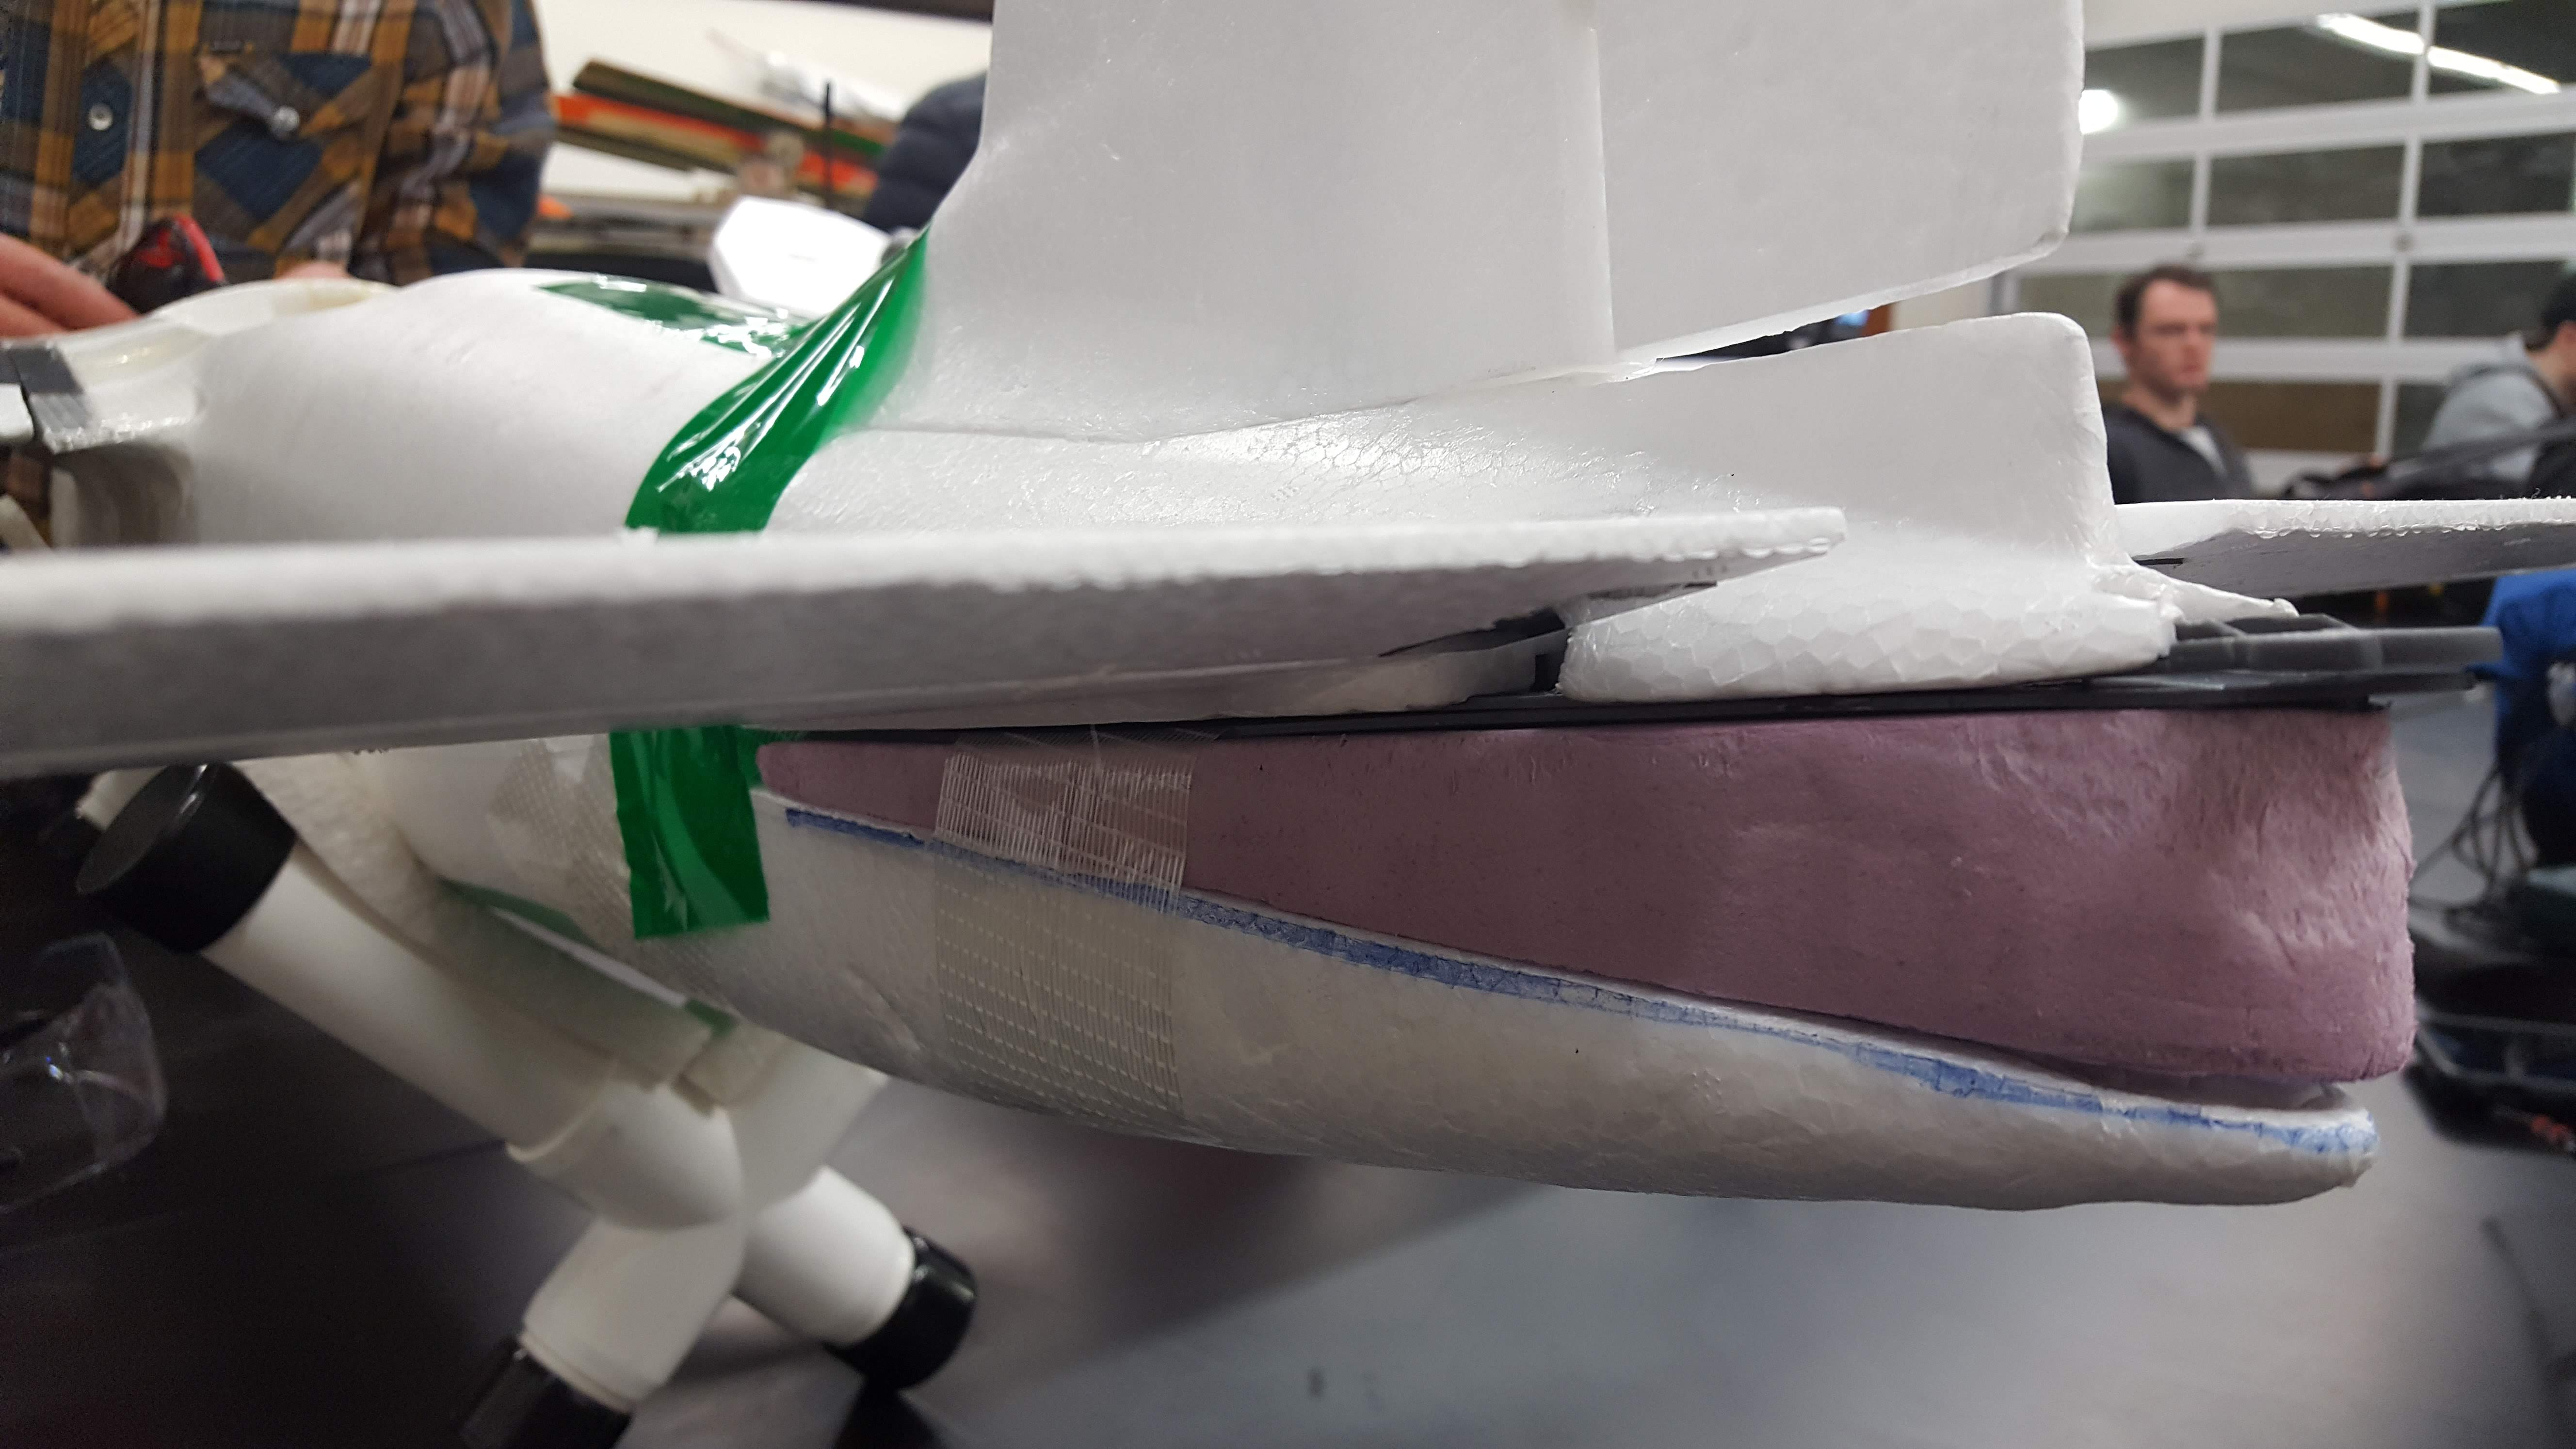
\includegraphics[width=\textwidth]{./figs/tailwedge.jpg}
\caption{The wedge finished and installed on the aircraft. Note that the outer surface of the wedge is flush with the outer surface of the aircraft's tail. It should be noted that the orientation of this image makes the wedge appear larger than it actually is---the angle is still 7.5°.}
\label{wedge}
\end{figure}

\section{Testing \& Validation}

Upon finishing construction we performed a flight test and trimmed the elevator in the new configuration. We were pleased to find that our predictions and analysis very closely matched the actual result as we needed zero deflection to trim the aircraft in this new configuration. Figure~\ref{deflect} shows the empennage after the flight were we trimmed the aircraft.

\begin{figure}[h]
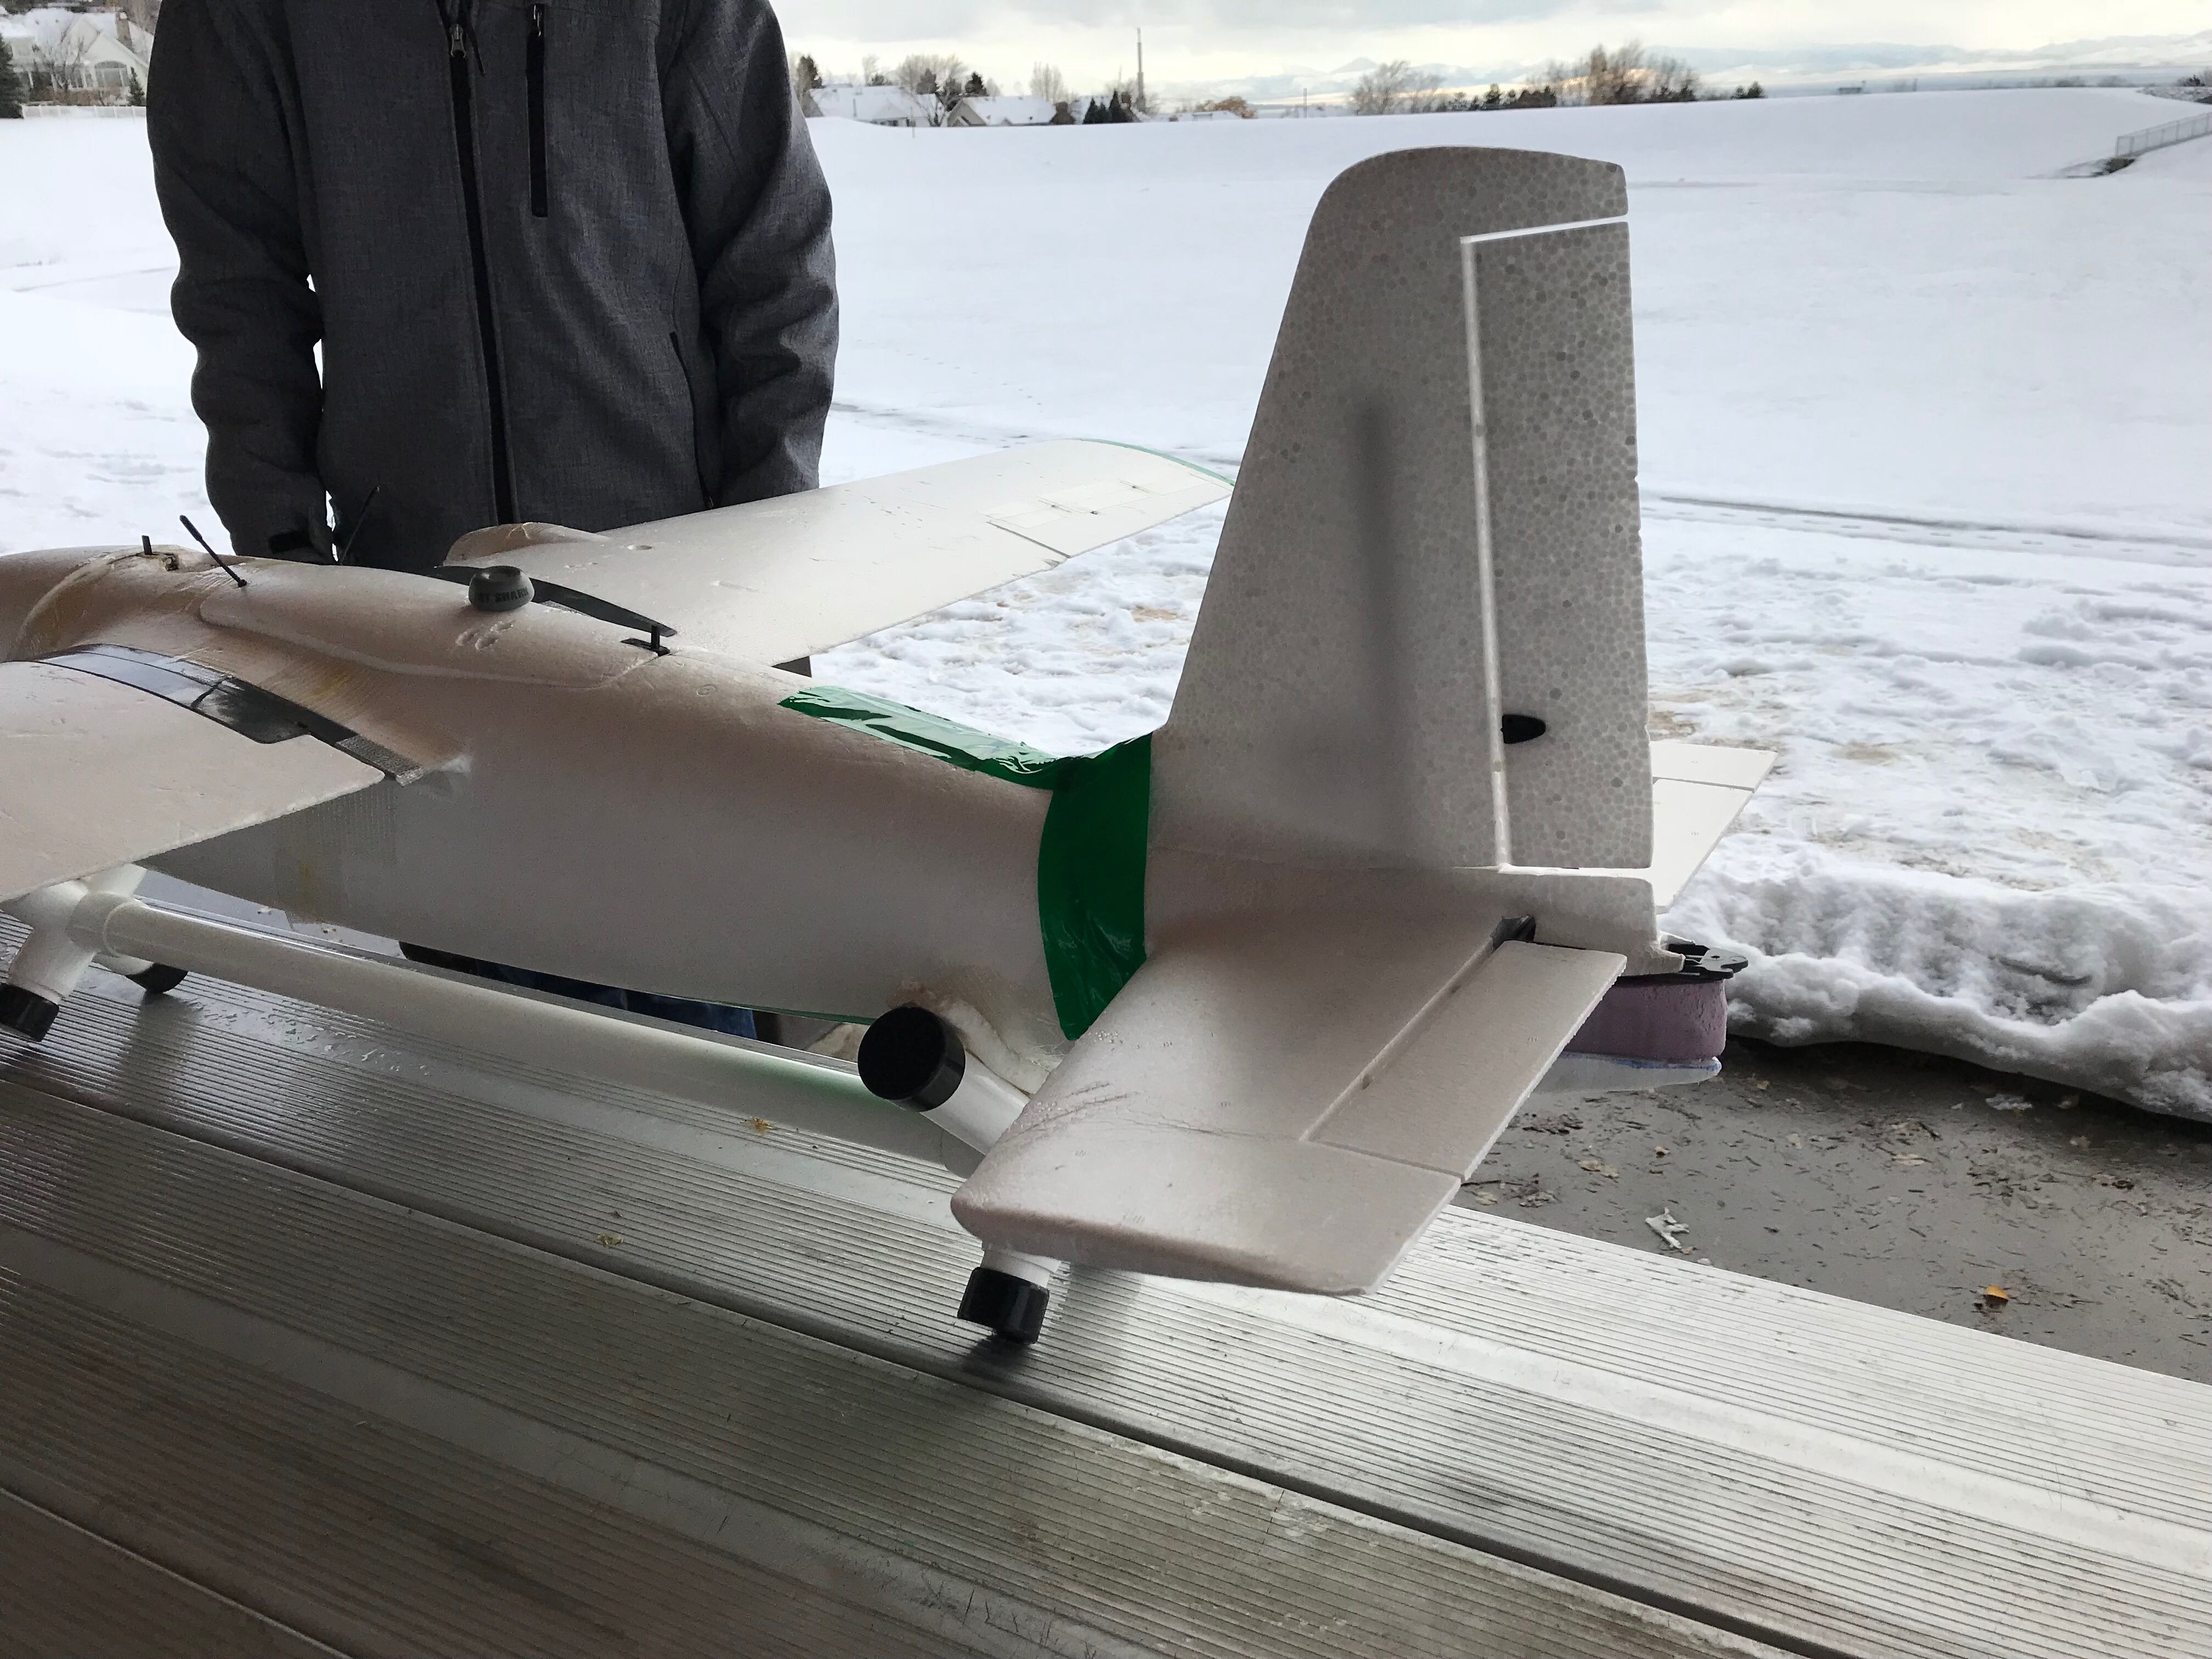
\includegraphics[width=\textwidth]{./figs/empennage.jpg}
\caption{The empennage after trimming the aircraft. As can be seen the deflection on the elevators is 0°, indicating that the wedge causes the correct incidence angle and negative lift.}
\label{deflect}
\end{figure}

\section{Conclusion}

We are very pleased with the implementation of this wedge as its success will aid in meeting our requirements and key success measures. Primarily, the wedge will mitigate the risk of saturating our elevator and thus crashing because we do not have the control authority to recover. This benefit has been captured in the failure modes and effects analysis that can be found in AF-007. Mitigating the chance of failure will allow all of our key success measures to be achieved. More specifically, the increased control authority will allow for increased precision in our flight path. This will help us decrease the number of obstacles hit and increase how close we get to waypoints.

\end{document}
